\section{Dirac Strings and Monopoles}
In order to progress these ideas to incorporate the overall picture of entire lattice it is necessary to motivate the language from the concepts of Dirac strings and monopoles. In his 1931 Paper entitled `Quantised Singularities in the Electromagnetic Field', Dirac postulated that the existence of magnetic monopoles would automatically imply that electric charge must be quantised, specifically that :
\par
\begin{equation}
    e = \frac{\hbar c}{2g} n \ ,
\end{equation}
\par
where $n = 0, \pm 1, \ \hdots $ e is the fundamental unit of electric charge and g is the magnetic charge of a monopole. {\cite{b1}}
\par
Dirac started with a pair of magnetic poles connected by an ideal string.  He then took one of the poles and sent it off to infinity.  What he was left with was a magnetic monopole who's magnetic flux was solely due to the string. This string could be shrunk to a line, thus becoming a remnant of one end of Coulomb's bar magnet. Dirac thus had produced an object that created the magnetic field of a single magnetic pole everywhere in space except on the string. This is known as a Dirac string.
\par
\begin{figure}[ht!]
    \begin{center}
        \subfloat[Classical bar magnet][Classical bar magnet]{
        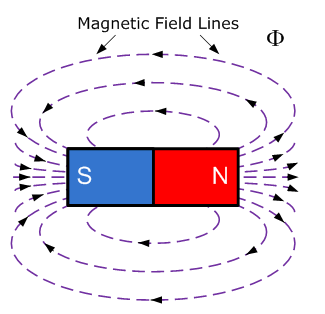
\includegraphics[width=0.30\textwidth]{mag2.png}
        \label{fig:sf8.1}}
\qquad
        \subfloat[Monopoles connected by a string][Monopoles connected by a string]{
        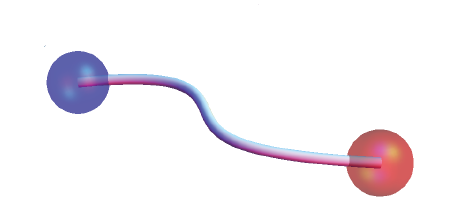
\includegraphics[width=0.40\textwidth]{monostring1.png}
        \label{fig:sf8.2}}
\qquad
        \subfloat[Dirac monopole][Dirac monopole]{
        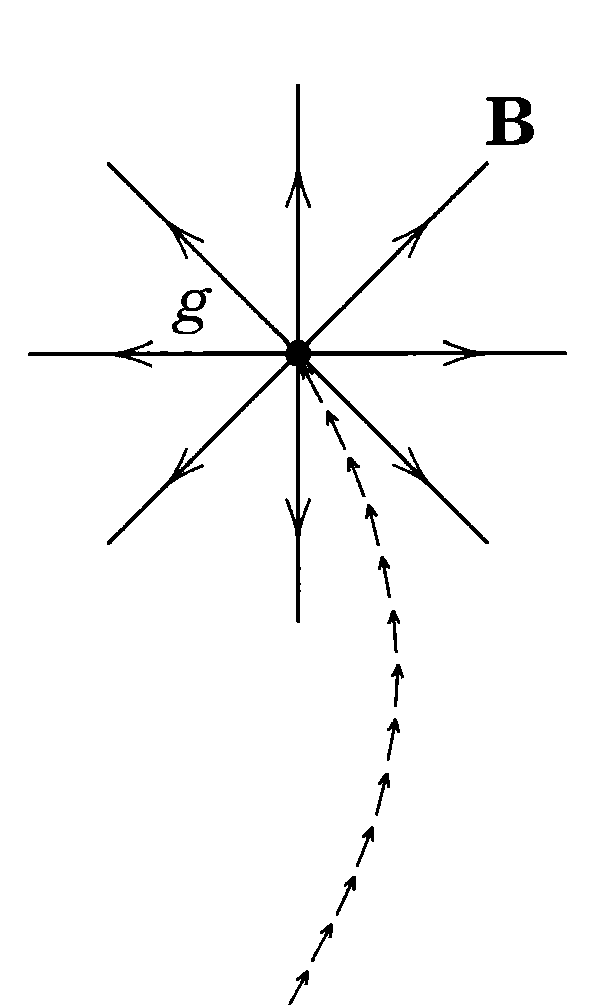
\includegraphics[width=0.15\textwidth]{diracmono.png}
        \label{fig:sf8.3}}
        \caption[Examples of types of magnets]{Examples of types of magnets}
        \label{fig:gf8}
    \end{center}
\end{figure}
The magnetic flux due to the monopole is exactly compensated by the flux fed into the monopole via the string, so the string is an inseparable part of Dirac's monopole. This means that the net flux through any closed surface is still zero, satisfying Maxwell's Equation $\Delta \cdot B = 0$.
\subsection{The Charge Model}
The islands interact via long-range pair wise dipolar interactions. There are two different, but equivalent, ways in which one can model the interactions between the islands, the pure dipole model and the charge model. The emergence of the quasi-particles is more easily seen in the charge formalization.
\clearpage
In the charge model the magnetic dipoles are imagined to be stretched into charged dumbbells which carry opposite charges, $\pm$q, at their ends. The magnitude of the charges are q $= \frac{\mu}{l}$, l is the length of the island. We then take the limit $l \rightarrow a$ , where a is the lattice spacing.  For the interaction between two vertices, given by the magnetic Coulomb law:
\par
\begin{alignat*}{3}
    &V(r_{\alpha \beta}) &&= \frac{\mu_{0}}{4\pi} \frac{Q_{\alpha} Q_{\beta}}{r_{\alpha \beta}} \,\,\, &&; \alpha \neq \beta \ , \label{eq:2} \tagaligneq \\
    &V(r_{\alpha \beta}) &&= \frac{1}{2} v_{0}Q_{\alpha}^{2} \,\,\, &&; \alpha = \beta \ , \label{eq:3} \tagaligneq
\end{alignat*}
\par
where $Q_{\alpha}$ is the total magnetic charge at vertex $\alpha$, $r_{\alpha \beta}$ is the distance between two vertices $\alpha$ and $\beta$ and $v_0$ is a 'self energy' resulting from the interaction of charges at the same vertex.
\subsection{Emergence of Fractional Quasi-particles}
When several Kagome base units are constructed into a lattice the magnetic monopoles may be realised as emergent fractional quasi-particles in the structure.  An important note to make here is that these fractional quasi-particles cannot be constructed out of combinations of the elementary particles, as opposed to quasi-particles like Cooper pairs which are a combination of two electrons.
\par
We get emergent `monopoles' due to the cooperation of base units which are arranged differently.  The emergence is unlike its components insofar as they are incommensurable but is instead a result of combinations of fractional parts of these base units. This meaning is easily seen when you look at an adjacent series of overturned dipoles.  The flipping of one dipole will change the two vertices it is contained by.
\par
The ground state of the Kagome lattice in which all dipoles point in one global direction, consists of vertices with $\pm$q net charge. If we now consider an excited state in which a continuous chain of dipoles(or charged dumb bell) has been flipped there will now at either end be a vertex of charge -3q marked in red and +3q for the vertex marked in blue.
\par
\begin{figure}[ht!]
    \begin{center}
        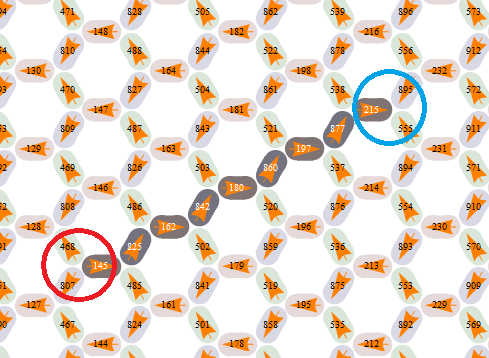
\includegraphics[width=0.4\textwidth]{stringkag.png}
        \caption[Overturned string of dipoles]{Two Monopoles connected by a string of overturned dipoles}
        \label{fig:gf9}
    \end{center}
\end{figure}
In the above Figure 10. the string of overturned dipoles is marked darker than it's surrounding dipoles.  The `charges' at the marked vertices can be viewed as a `monopole-antimonopole' pair interacting via the magnetic Coulomb interaction given by the equations 2 \& 3.
\clearpage
